\chapter{Implementation}
The project is programmed through HTML, CSS, JavaScript, PHP and MySQL. HTML, CSS and JavaScript are responsible for the front end which includes presentation of web page and every click event handling. The back end data is processed by PHP which actually interacts with database. In this chapter, how every key functionary is achieved by code will described.
\section{Instruction Page}
Instruction page provides information about the migration game and it is also a registering entrance. In general, this page is implemented by HTML and PHP. Paragraphs are clear with 18 pixel font size, informing what users can do during the game. Registering part has connection with database, inserting user information . All typed content would be validated by testing whether they are empty (Listing 4.1). Whichever is empty, an alert window will pop up and the cursor will focus on where is empty.
%\begin{figure}[!htb]
	%\centering
	%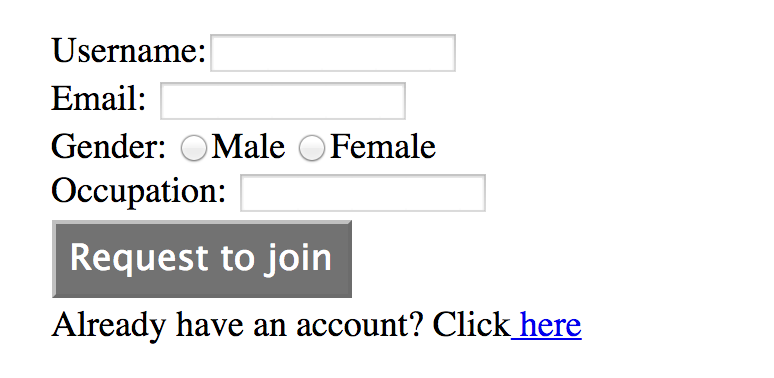
\includegraphics[width=8cm]{register}
	%\caption{Register segment}
	%\label{Figure:figRgst}
%\end{figure}

\begin{lstlisting}[caption=User data validation segment]
function inputCheck(registerForm){
	if(registerForm.username.value==""){
		alert("Please enter your username.");
		registerForm.username.focus();
		return(false);
	}
	if(registerForm.email.value==""){
		alert("Please enter your email.");
		registerForm.email.focus();
		return(false);
	}
	if(registerForm.occupation.value==""){
		alert("Please enter your occupation.")
		registerForm.occupation.focus();
		return(false);
	}
}

\end{lstlisting}
Eventually, the instruction page is implemented like \fref{Figure:intro}. Instruction of this game is described from the top and at the bottom of this page, there is a registering component. A style of "hover" is added in the button, so that when the mouse moves upon the button, the colour will be changed.
\begin{figure}[!htb]
  \centering
  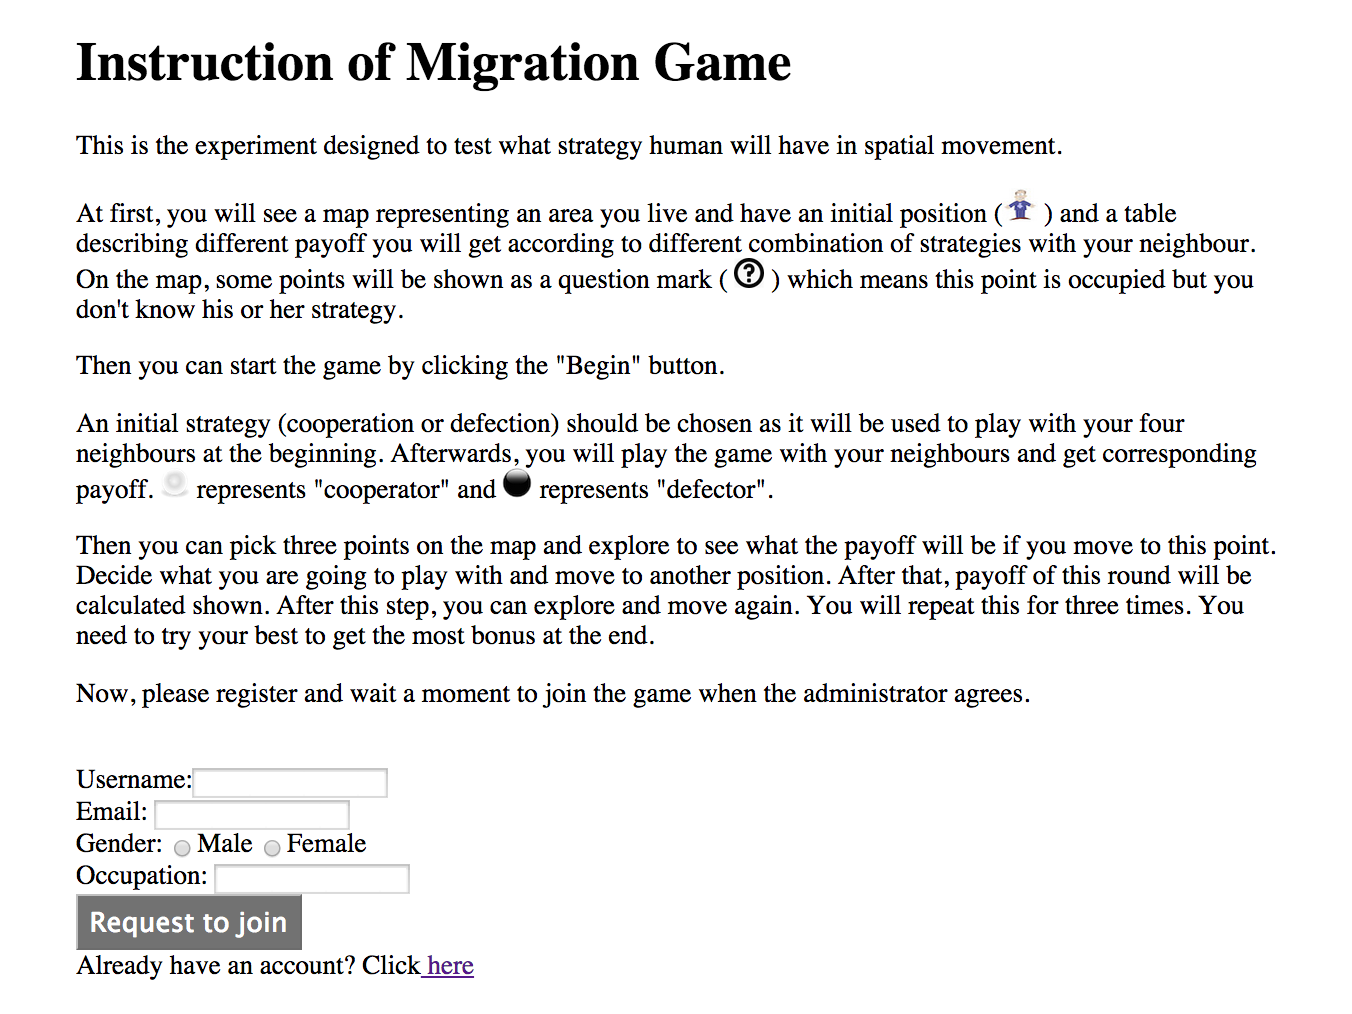
\includegraphics[width=14cm]{instruction.png}
  \caption{Intstruction page}
  \label{Figure:intro}
\end{figure}


\section{Log On Page}
The log on page of users is similar to that of administrators which has two labels of an administrator's name and the password, enclosed by a $\langle legend \rangle$ element. Every time a manager logs in, a SQL query like \textit{"SELECT id FROM admin WHERE adminname='\$adminname' AND password='\$password'" }will be executed. If it fails, the person can try again.

\section{Administrator Page}
\subsection{User List}
To make the page more efficient, "Ajax" is used in order not to refresh the whole page every time an option is selected. The source code is presented in Listing 4.2 which is called when the value of the $\langle select \rangle$ element that includes values of "all users", "users on request" and "users agreed" is changed. Relevant records in the "user" table will be chosen and displayed as a table which is completed in a php file - "getuser.php". In the "getuser.php" file, a specific table is exhibited by selecting users according to the "state" value and using "echo" to output.

\begin{lstlisting}[caption=Ajax segment for listing users]
function showUser(str){
		if (str=="") {
    		document.getElementById("txtHint").innerHTML="";
  		  	return;
  		} 
  		if (window.XMLHttpRequest) {
    		// code for IE7+, Firefox, Chrome, Opera, Safari
    		xmlhttp=new XMLHttpRequest();
  		} else { // code for IE6, IE5
    		xmlhttp=new ActiveXObject("Microsoft.XMLHTTP");
  		}
  		xmlhttp.onreadystatechange=function() {
    		if (xmlhttp.readyState==4 && xmlhttp.status==200) {
      			document.getElementById("txtHint").innerHTML=xmlhttp.responseText;
    		}
  		}
  		xmlhttp.open("GET","getuser.php?q="+str,true);
  		xmlhttp.send();
	}

\end{lstlisting}

\subsection{User Management}
Administrators have the right to control the game or the application, therefore some operations against users should be accomplished. In this project, an manager can administrate users by deleting and approving.

If a user is disagreed to take part in the game, he or she could be deleted. In the listed table of players, deletion is one of the two activities for each individual. When this button is clicked, a new URL will be generated by adding the user id value which would be deleted at the end and direct to another php file which interacts with the real database. A "delete" query will be activated which should be \textit{"DELETE FROM user WHERE uid='\$uid'"}. The "uid" value can be obtained through URL.

A password can be sent to a user by email by the "email" button is clicked. There are two key problems to be solve. How to pass the value of who needs to agree is the first question and the solution is pass necessary values through URL. When a user is approved, the user id will be put at the end of the url, thus the php can know whose email is going to be sent to and then execute it. In addition, two package are imported for email sending which are "class.phpmailer.php" and "class.smtp.php". They are open source in the Internet and specify to securely send an email by SMTP. As shown in Listing 4.3, both of them are required and then it configures some fundamental variables such as host address, SMTP username and password. After email sent, the 9-digit randomly generated password will be encrypted by MD5 and saved in the "user" table and update state of the user into "1" which means having been agreed.
\begin{lstlisting}[caption=Email segment]
require ('class.phpmailer.php');
require ('class.smtp.php');

$mail = new PHPMailer;
$mail->isSMTP();                                      // Set mailer to use SMTP
$mail->Host = 'smtp.gmail.com';  // Specify main and backup SMTP servers
$mail->Port = 465;
$mail->SMTPAuth = true;                      // Enable SMTP authentication
$mail->Username = '$my email address';                 // SMTP username
$mail->Password = '$my email password';                  // SMTP password
$mail->SMTPSecure = 'ssl';                // Enable encryption

$mail->From = 'kevininsoton@gmail.com';
$mail->FromName = 'admin';
$mail->addAddress($email);     // Add a recipient

$mail->addReplyTo('huntingkevin89@gmail.com');
$mail->WordWrap = 50;

$mail->IsHTML(true);    // set email format to HTML
$mail->Subject = "Migration game password";
$mail->Body = "Welcome to migration game! Your password is ".$password.". Please use it to log in the game.";

\end{lstlisting}

The administrator's page is displayed in \fref{Figure:admin} which contains a drop-down list choosing among different users' types - on request and agree. The result is listed below, with some information of every user. The administrator can delete which means reject here, and email or approve.
\begin{figure}[!htb]
  \centering
  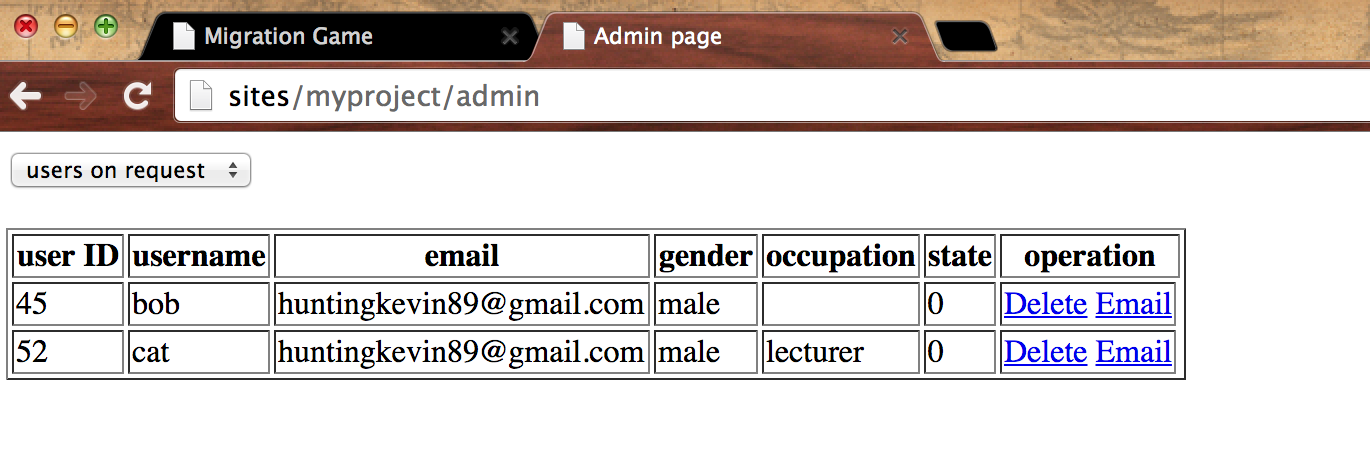
\includegraphics[width=14cm]{admin.png}
  \caption{Administrator page}
  \label{Figure:admin}
\end{figure}

\section{Game Page}
Game page is definitely the core of the application. Final interface is illustrated in the appendix. As the design described in Chapter 3, the project has two main classes to build the game page. The PHP file "login .php" is to test whether the user is in the database and if it matches, HTML page will be loaded. For log on component, it is accomplished as Listing 4.4 shows. If the post command is not "post", it will exit alerting that it is an invalid access in order to make sure there is only one entrance to enter the game. People cannot play the game by just using the url, but instead, entering through log on window is necessary. Otherwise a warning would be shown. The page is programmed by "echo" and using html syntax. 
\begin{lstlisting}[caption=Code of log on component]
if(!isset($_POST['submit'])){
        exit('Invalid access!');
    }
    
    $username = $_POST['username'];
    $password = md5($_POST['password']);

    //connect to database
    include('conn.php');
    // check if user exists
    $sql="select uid from user where username='$username' and password='$password'";

\end{lstlisting}

To make the page clearer, the html page is split into three divisions - \textit{information, chessboard and operation}. Information block contains a begin button which should be clicked to start the game and a textarea below to display on which step the user is and provide guidance. The prisoner's dilemma matrix which is created using a $\langle table \rangle$ element and icon representation are displayed at the end of this division. 

The chessboard division is a table with double borders so that it can be more stereoscopic. What is more, in order to set the cross of two lines as a point that can be placed other elements  like black and white chesses, this web application creates $\langle i \rangle$ elements whose class name are called "iBox" and configures in the stylesheet to fix every position of $\langle i \rangle$ components. To generate them, the project utilises some basic interface classes such as "addClass" and "createElement" in JavaScript. In Listing 4.5, an $\langle i \rangle$ element is created and set the style left and top value as i and j increase, then it is given an id. Additionally, building a map should have an array to know which point is empty or occupied. In this development, 50 random indexes are assigned as defectors or cooperators and the rest are undefined which means they are vacant. If one point is occupied, it will have a question mark covered on it. Eventually, the initial location of the player is fixed, but neighbours are random as well.

\begin{lstlisting}[caption=Part of code to create a map]
iBox=document.createElement("div");
	iBox.className="iBox";
	for(var i=0;i<10;i++)
		for(var j=0;j<10;j++){
			var iObj=document.createElement("i");
			iObj.appendChild(document.createTextNode(i*10+j));
			iObj.style.left=j*41+1+"px";
			iObj.style.top=i*41+1+"px";
			iObj.id=i*10+j;
			iObj.className="piece";
			iBox.appendChild(iObj);
			iArray.push(iObj);
	}

\end{lstlisting}


To make the page as simple as possible, the operation division is implemented as a three-layer wrapper which can be seen in Listing 4.6. In $\langle form \rangle$, because every bottom element has a style setting that padding-bottom is 330 pixels, only one $\langle div \rangle$ can be seen one time. The "step1" has a button that links to "step2" so that when the button is pressed, "step1" will disappear and just "step2" is visible. This simplicity can be concise and friendly enough for users to manipulate during the game.
\begin{lstlisting}[caption=Part of the code to wrap elements]
<div id="form_main_wrapper">
                <div id="form_main">
                    <div id="form_content">
                    	<div id="step1" style="padding-bottom: 330px">...</div>
                    	<div id="step2">...</div>
                    	...

\end{lstlisting}

The second problem is how to handle every click event and make the game procedure go fluently. For the click on the map, jQuery is used to listen to every element. As can be seen in Listing 4.7, when element of "i.piece" is clicked, the function will be activated. If tMove which counts the step for a user to move is less than one, the class name will be changed to "piece man" which is defined in the stylesheet to add the man picture on the point and remove the picture of previous location by deleting "man" from the class name. Furthermore, it calculates the coordinate of the clicking position and save it in a invisible element. It is similar for the method to explore three locations except one thing. Exploring needs to calculate the payoff of the point at the same time, so a local variable is created to remember the total bonus computed according to the prisoner's dilemma matrix. Then the value is saved in a hidden element.

\begin{lstlisting}[caption=Part of the code to move the player]
function movePlayer(){
	$("i.piece").click(function(){
		if(tMove<1){
			tMove++;
			if(iPoint[this.id]==undefined){
				var pieceObj=document.getElementById(this.id);
				var manObj=document.getElementsByClassName("piece man")[0];
				manObj.className="piece";
				pieceObj.className="piece man";
				var x=this.id%10;
				var y=parseInt(this.id/10);
				pPosition=this.id;
				pxy="("+x+","+y+")";
			}
                    	...

\end{lstlisting}

Buttons in the operation division includes strategy choice of cooperation and defection. However, the most important clicking event of this segment is the "continue" button which connects to the next step to make the whole game run influently. It is achieved by the method \textit{"window.location.href"}.

The game page is finally implemented as \fref{Figure:game}. Information module is on the left and in the middle is the chessboard-like lattice. Users can operate from the operation module on the right of the window.
\begin{figure}[!htb]
  \centering
  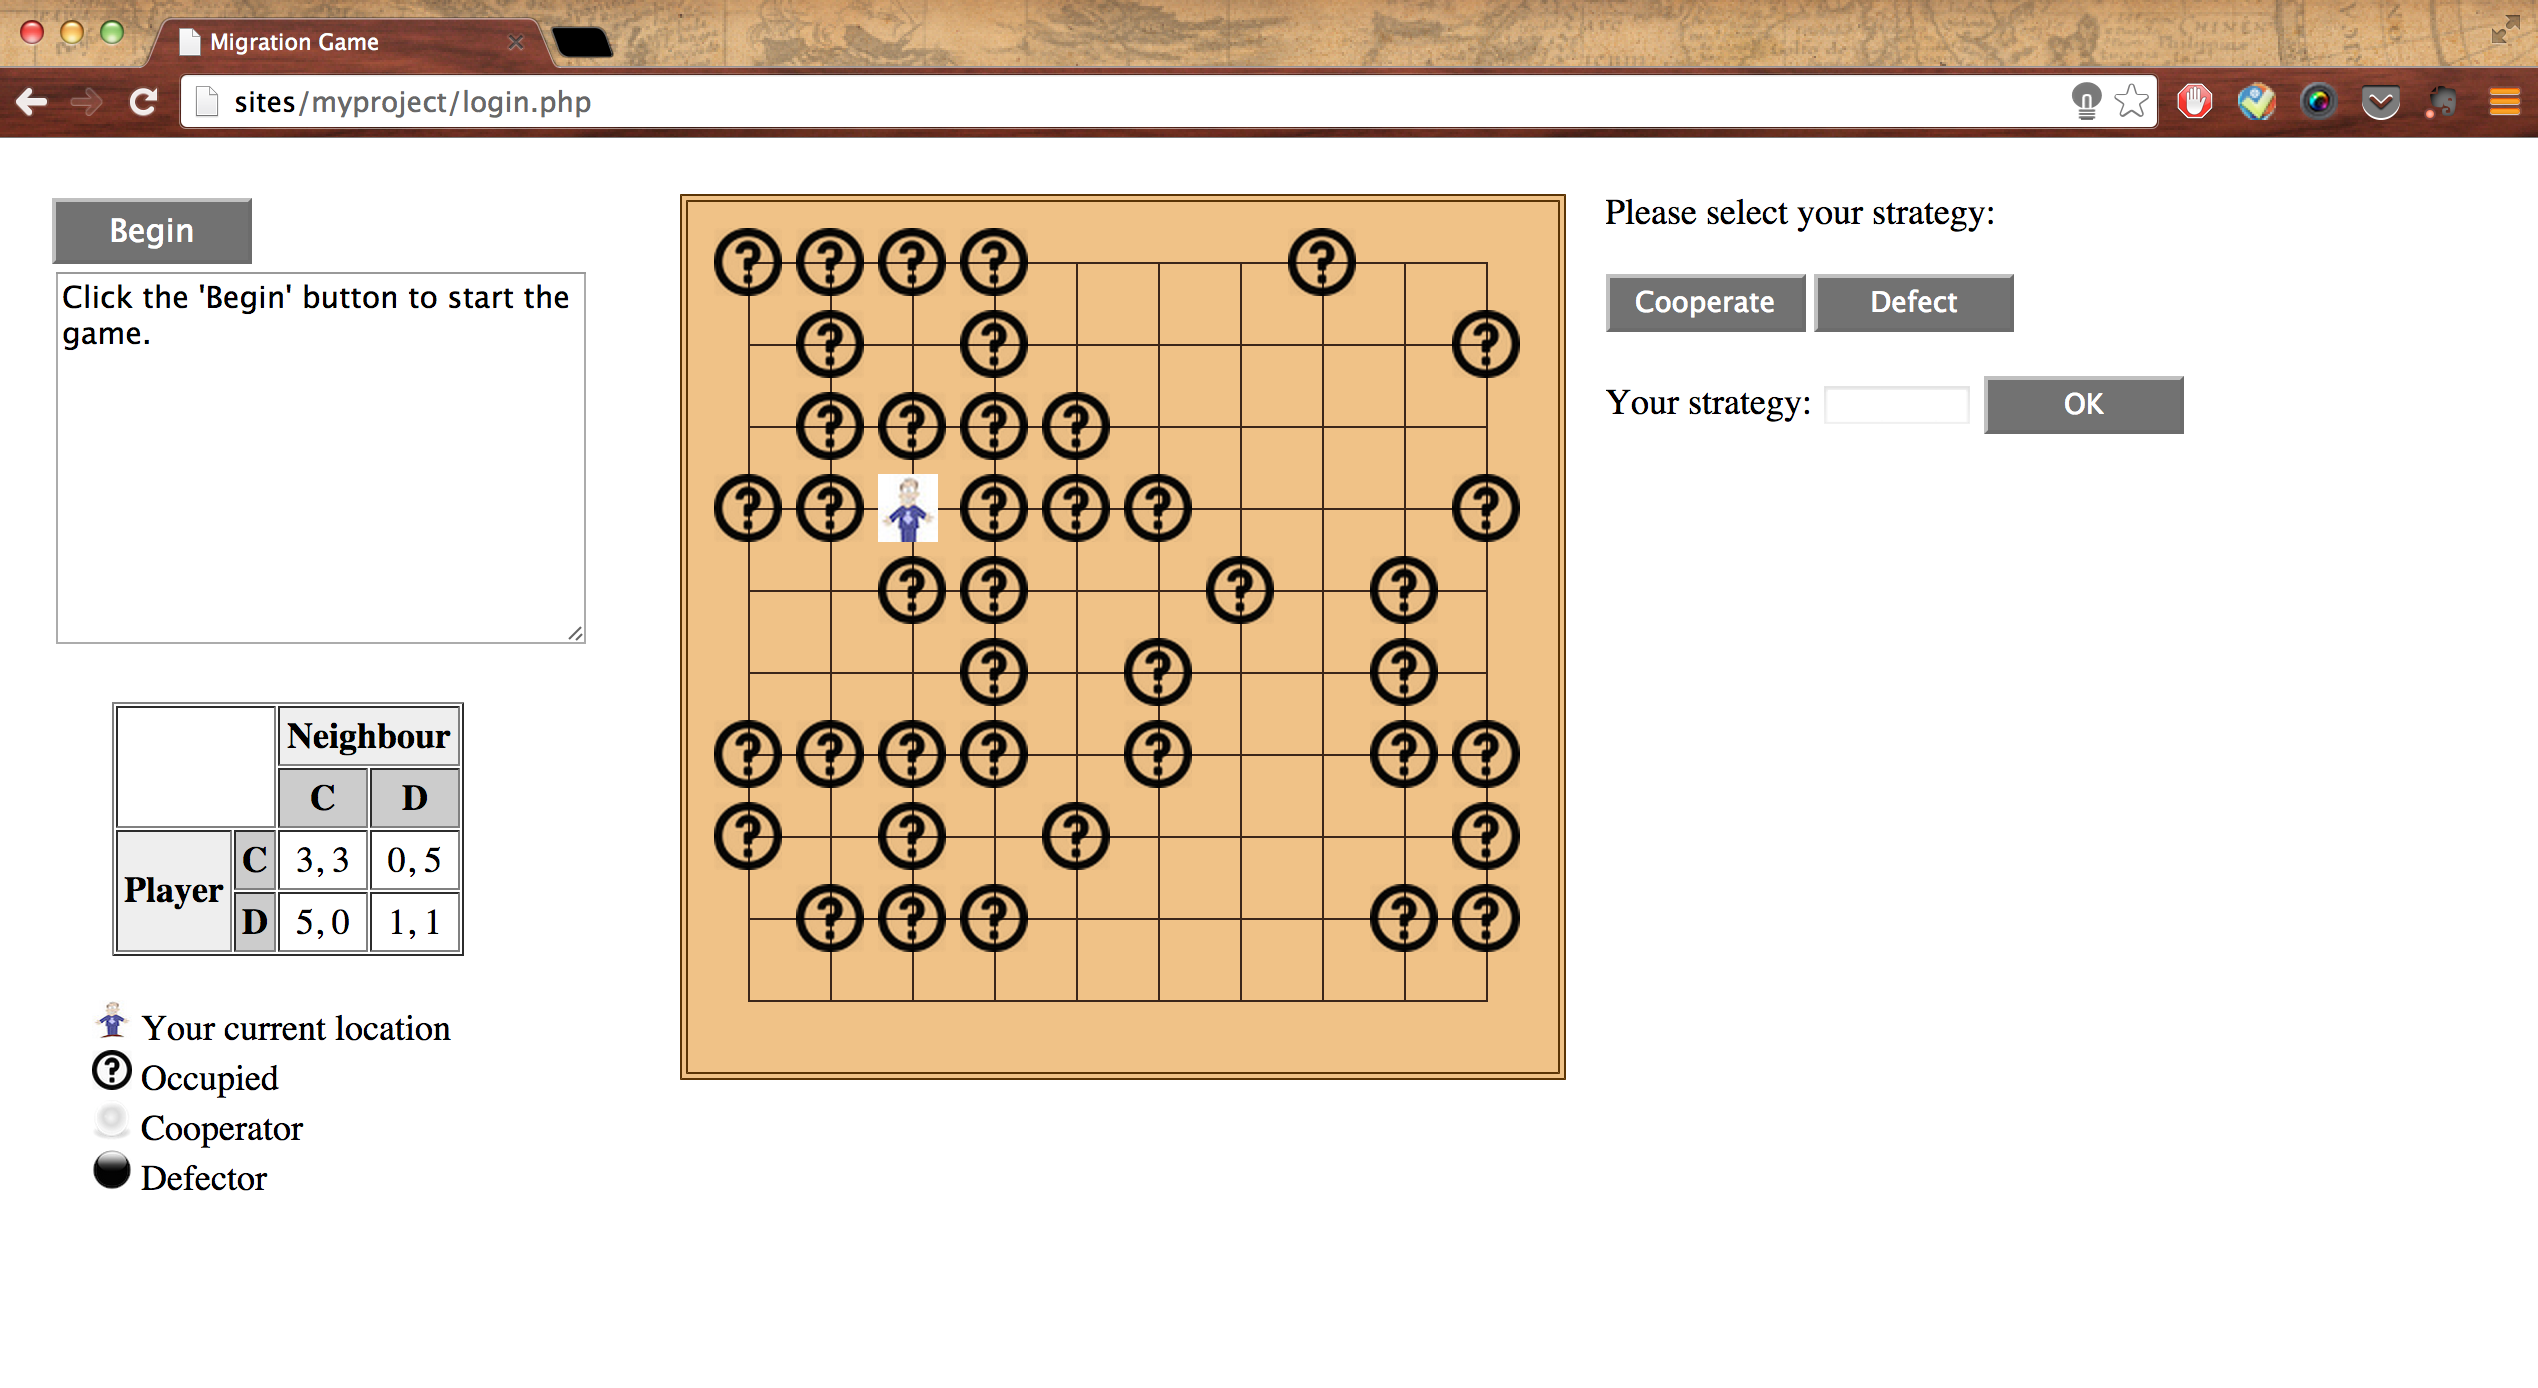
\includegraphics[width=14cm]{game.png}
  \caption{Game page}
  \label{Figure:game}
\end{figure}

Finally, when a game ends, results will be shown by getting data from database of the final record.

\section{Database Operation}
To provide operation of database, connection between front end and back end should be built at first which is written in PHP. To be specific, the project uses "mysql connect" function to create link and "mysql select db" to choose an exact database. In HTML, every component which needs to communicate with database would be programmed in a $\langle form \rangle$ element and deliver data by "post" method. When data is submitted, the page would direct to the corresponding php file and pass the data. Different SQL queries of select, update, insert and delete are used. Select query is for administrators' and users' name and password check, and once a requesting user is approved, updating sentence is run for saving password and change state value. Moreover, when a new user registers and a new game record is ready to save, data will be inserted. Deleting action is just for database management if a user is not agreed.

Many hidden elements are used in the game page as to temporarily save helpful data during the game. For instance, when a user clicks an empty point to explore, the coordinate and its payoff will be calculated and stored in an invisible component. When data is eventually submitted, all information in these elements will delivered at the same time.

Data lists stored in database consist of user, administrator and game record. Part of stored data is shown in \fref{Figure:record}.
\begin{figure}[!htb]
  \centering
  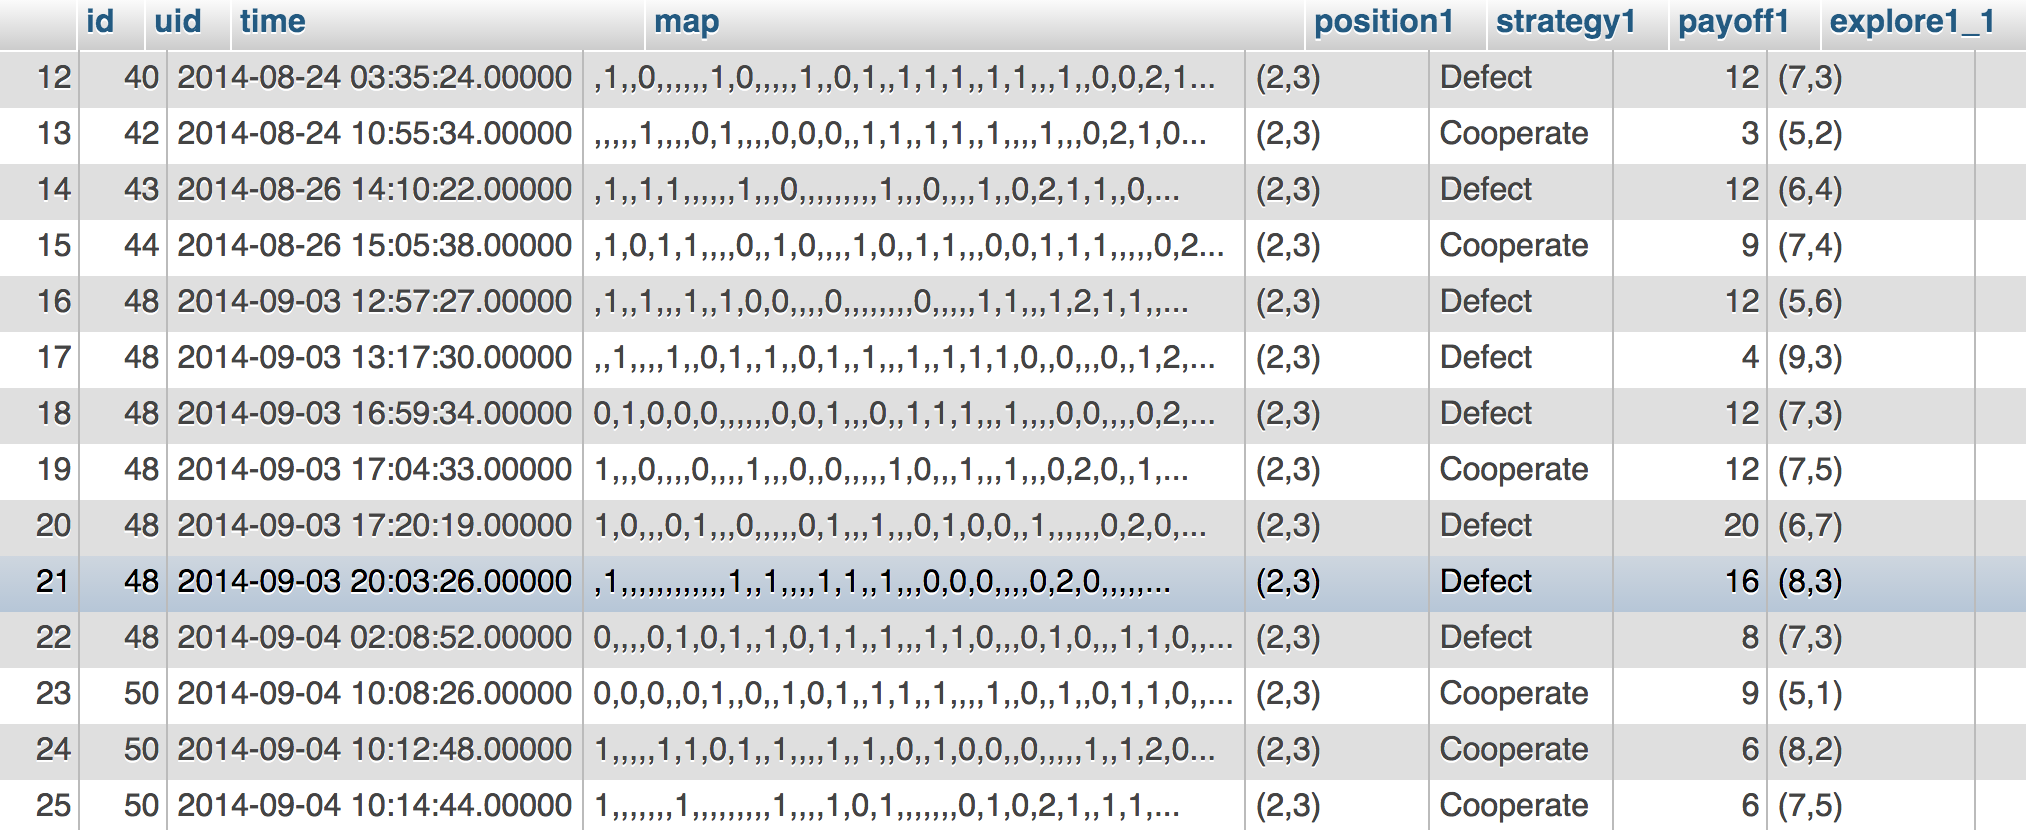
\includegraphics[width=14cm]{recordtable.png}
  \caption{Part of record table}
  \label{Figure:record}
\end{figure}
